\chapter{Tiling and Unrolling Optimizations\label{chap:optimizations}}

Cache tiling is a classic performance optimization that exploits temporal reuse of data to get maximal benefit from data caches~\cite{Lam91, Wolf91}.  Many numerical computations, including e.g.~dense matrix multiplication, involve significant data reuse due their all-to-all computational pattern.

\begin{lstlisting}[frame=single, label=untiledmm, caption={Untiled Matrix Multiply}, belowskip=0.5em]
for i in range(numRows):
  for j in range(numCols):
    C[i,j] = 0
    for k in range(rowLen):
      C[i,j] += A[i*rowLen + k] * \
                B[j*rowLen + k]
\end{lstlisting}

For example, consider the code for matrix multipication given in Listing \ref{untiledmm}, with a vizualation of the elements accessed to compute a single output value shown in Figure \ref{untiled_diagram}.  If the \lstinline{A} and \lstinline{B} matrices are large, then this code will have poor cache behavior and thus suboptimal performance.  To understand why, consider the data access pattern.  The columns of \lstinline{B} are accessed repeatedly, and thus could benefit from being cached to lower their access times.  However, between each access to an element of \lstinline{B}, the entire rest of \lstinline{B} is accessed, in addition to an entire row of both \lstinline{A} and the output matrix and.  Thus the column of \lstinline{B} will be evicted from the cache between each use, and it will have to be read from a slower level of the memory hierarchy.  Things are similar with the rows of \lstinline{A}.

A better access pattern is one that accesses pieces (called tiles) of the input data at a time such that as much data as possible remains resident in cache between subsequent uses.  Consider the vizualation of a tiled organization of matrix multiply in Figure \ref{tiled_diagram}.  The rows of the \lstinline{A} matrix are grouped into tiles, and each \lstinline{A} tile is entirely consumed before moving onto the next one.  An analagous grouping is done with \lstinline{B}'s columns.  Finally, the iteration through each group of rows and columns is broken up into tiles as well.  Code for this tiling is given in Listing \ref{untiledmm}, where we see that each loop in the original code is broken up into both an outer loop that iterates across tiles and an inner loop that iterates across elements of the current tile.

Consider the data access pattern in this version.  Now rather than the entire matrix \lstinline{B} being accessed between each access to a given element of \lstinline{B}, only an entire \emph{tile} of \lstinline{B} is accessed.  If the tile size is small enough that this tile fits in cache, subsequent accessed to elements of \lstinline{B} will be much faster in this version.  The tile size that works best depends on the size of the cache, the size of the data, and the particular code being executed.

\begin{figure}
\centering
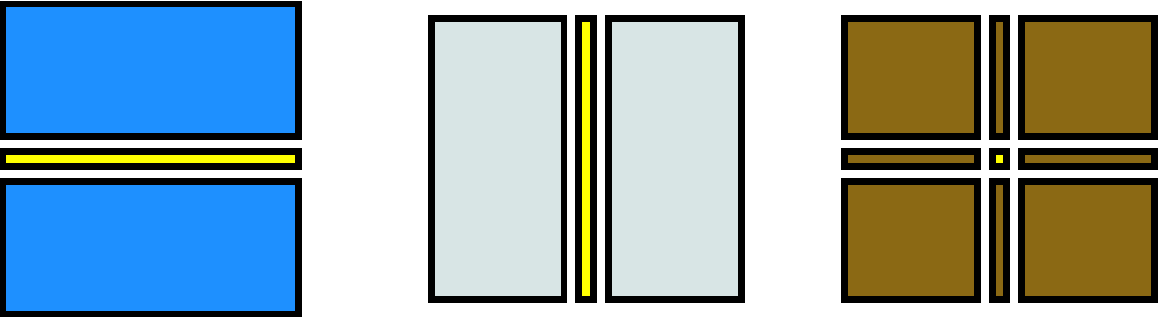
\includegraphics[scale=0.4]{UntiledMMIterationSpace.pdf}
\caption{Untiled Matrix Multiply Iteration Order}
\label{untiled_diagram}
\end{figure}

\begin{figure}
\centering
\includegraphics[scale=0.4]{TiledMMIterationSpace.pdf}
\caption{Tiled Matrix Multiply Iteration Order}
\label{tiled_diagram}
\end{figure}

\begin{lstlisting}[frame=single, label=tiledmm, caption={Tiled Matrix Multiply}, belowskip=0.5em]
for at in range(0, numRows, atSize):
  for bt in range(0, numCols, btSize):
    for i in range(at, at+atSize):
      for j in range(bt, bt+btSize):
        C[i,j] = 0
    for kt in range(0, rowLen, ktSize):
      for i in range(at, at+atSize):
        for j in range(bt, bt+btSize):
          for k in range(kt, kt+ktSize):
            C[i,j] += A[rowLen*i + k] * \
                      B[rowLen*j + k]
\end{lstlisting}

Cache tiling need not be for a single level of cache; tiling loops can be added for each level of cache in which to keep data resident between accesses.  In addition, tiling can be used to keep data resident in other levels of the memory hierarchy such as registers.

There has been much work on automating the process of tiling, including both generating the outer tiled loops from the inner ones as well as automating tile size selection given a tiled loop nest~\cite{Lam91, Wolf91} (REFS).  It might appear at first glance that determining good tile sizes for a given loop nest might be easy to do analytically.  Much work has been done on designing analytic models to estimate good tile sizes~\cite{Cole95, Shir12, Yoto03, Yoto05}.  However, while these models often perform fairly well, the state of the art for achieving the best performance is still offline autotuning to find the best settings for a particular target architecture, even for a problem as well-studied as matrix multiplication~\cite{Whal00}.

